\documentclass[11pt,a4paper]{article}

% ---------- Kodlama, dil ve tipografi ----------
\usepackage[utf8]{inputenc}
\usepackage[T1]{fontenc}
\usepackage{lmodern}
\usepackage[turkish,shorthands=off]{babel}
\usepackage{microtype}

\usepackage[margin=2.5cm,headheight=15pt]{geometry}
\usepackage{xcolor}
\usepackage{titlesec}
\usepackage{enumitem}
\usepackage{array}
\usepackage{booktabs}
\usepackage{tabularx}
\usepackage{float}
\usepackage{graphicx}
\usepackage{listings}
\usepackage{mdframed}
\usepackage{pifont}
\usepackage{parskip}
\usepackage{fancyhdr}

% ---------- Renk tanimlari ----------
\definecolor{accent}{RGB}{150,72,38}
\definecolor{darkgray}{RGB}{90,90,90}
\definecolor{lightgray}{RGB}{245,245,245}
\definecolor{codebg}{RGB}{30,30,30}
\definecolor{codetext}{RGB}{220,220,220}
\definecolor{codekw}{RGB}{240,160,90}
\definecolor{codecmt}{RGB}{125,165,120}
\definecolor{okgreen}{RGB}{35,120,55}

\definecolor{stTodo}{RGB}{115,115,115}
\definecolor{stInProgress}{RGB}{40,110,180}
\definecolor{stReview}{RGB}{200,130,20}
\definecolor{stMerged}{RGB}{120,60,160}
\definecolor{stDeployed}{RGB}{30,140,90}
\definecolor{stTest}{RGB}{205,95,35}
\definecolor{stDone}{RGB}{35,110,55}

% ---------- Baslik ve sayfa bicimi ----------
\titleformat{\section}
  {\Large\bfseries\color{accent}}{\thesection}{0.8em}{}
\titlespacing*{\section}{0pt}{2.0ex plus .4ex}{1.0ex}
\titleformat{\subsection}
  {\large\bfseries\color{accent!80!black}}{\thesubsection}{0.7em}{}

\pagestyle{fancy}
\fancyhf{}
\fancyhead[L]{\footnotesize\sffamily\color{darkgray}Ticket Manager}
\fancyhead[R]{\footnotesize\sffamily\color{darkgray}\nouppercase{\leftmark}}
\fancyfoot[C]{\footnotesize\sffamily\color{darkgray}---~\thepage~---}
\renewcommand{\headrulewidth}{0.8pt}
\renewcommand{\headrule}{{\color{accent}\hrule width\headwidth height \headrulewidth}}

\setlist{itemsep=2pt,parsep=0pt,topsep=4pt}
\emergencystretch=1em
\raggedbottom

% ---------- Yardimci komutlar ----------
\newcommand{\ok}{\textcolor{okgreen}{\ding{51}}}
\newcommand{\hayir}{\textcolor{darkgray}{\ding{55}}}
\newcommand{\statusbadge}[2]{%
  \colorbox{#1}{\makebox[3.0cm][c]{\color{white}\sffamily\bfseries\small #2}}}

% ---------- Kod listeleme bicimi ----------
\lstdefinestyle{sql}{
  language=SQL,
  backgroundcolor=\color{codebg},
  basicstyle=\ttfamily\footnotesize\color{codetext},
  keywordstyle=\color{codekw}\bfseries,
  commentstyle=\color{codecmt}\itshape,
  stringstyle=\color{codetext},
  numbers=left,
  numberstyle=\tiny\color{darkgray},
  numbersep=8pt,
  frame=none,
  breaklines=true,
  showstringspaces=false,
  tabsize=2,
  xleftmargin=2.6em,
  framexleftmargin=1.6em,
}
\lstdefinestyle{html}{
  language=HTML,
  backgroundcolor=\color{codebg},
  basicstyle=\ttfamily\footnotesize\color{codetext},
  keywordstyle=\color{codekw},
  commentstyle=\color{codecmt}\itshape,
  stringstyle=\color{codetext},
  numbers=left,
  numberstyle=\tiny\color{darkgray},
  numbersep=8pt,
  frame=none,
  breaklines=true,
  breakindent=1.5em,
  showstringspaces=false,
  tabsize=2,
  xleftmargin=2.6em,
  framexleftmargin=1.6em,
}
\lstset{style=sql}

% ---------- PDF meta (ASCII guvenli) ----------
\usepackage[unicode,colorlinks=true,linkcolor=accent,urlcolor=accent,citecolor=darkgray]{hyperref}
\hypersetup{
  pdftitle={Ticket Manager - Sistem Mimarisi ve Veritabani Tasarimi},
  pdfauthor={Ekin},
  pdfsubject={Sistem Mimarisi ve Veritabani Tasarimi},
  pdfkeywords={ticket manager, task management, cloudflare, d1, drizzle, better-auth, resend},
}

\begin{document}

% ============================================================
% KAPAK
% ============================================================
\begin{titlepage}
\centering
\vspace*{2cm}
{\color{accent}\rule{0.6\textwidth}{1pt}}
\vspace{0.8cm}

{\Huge \bfseries Ticket Manager\par}

\vspace{0.4cm}
{\Large \color{darkgray} Sistem Mimarisi ve Veritabanı Tasarımı\par}

\vspace{0.8cm}
{\color{accent}\rule{0.6\textwidth}{1pt}}
\vspace{1.2cm}

{\large \itshape Sıfır maliyetli ve öz-sunumlu (self-hosted); PlannedLost'un geliştirme\\
takibi ve diğer projelerin yönetimi için kurum içi Jira / Linear alternatifi\par}

\vspace{2cm}
{\normalsize
\begin{tabular}{rl}
\textbf{Tarih:}     & \today \\
\textbf{Sürüm:}     & v0.5 \\
\textbf{Hazırlayan:}& Ekin \\
\textbf{Durum:}     & Aktif Mimari Taslak \\
\end{tabular}\par}
\vfill
\end{titlepage}

\pagenumbering{roman}
\tableofcontents
\newpage
\pagenumbering{arabic}

% ============================================================
\section{Sistem Bileşenleri ve Teknoloji Seçimleri}

Ticket Manager; \textbf{PlannedLost}'un geliştirme sürecinin daha rahat
ilerlemesi ve kolay takip edilmesi, aynı zamanda diğer projelerin de tek
noktadan yönetilebilmesi için geliştirilen bağımsız bir görev takip
sistemidir. Harici servislere bağımlı kalmadan, sıfır maliyetle ve tam
yetki kontrolüyle çalışır. Uzun vadeli amaç;
\href{https://linear.app/}{Linear} gibi araçların ücretli özelliklerini
kendi sunucumuzda çalıştırarak lisans maliyeti olmadan sunan bir
alternatif oluşturmaktır. Bu hedefe uygun olarak seçilen bileşenler
aşağıda özetlenmiştir.

\begin{table}[H]
\centering
\small
\begin{tabularx}{\textwidth}{p{2.6cm}p{4.6cm}X}
\toprule
\textbf{Katman} & \textbf{Teknoloji} & \textbf{Gerekçe}\\
\midrule
Arayüz        & React + TypeScript            & Kanban tahtası gibi bileşenlerin tip güvenli ve performanslı çalışması.\\
\addlinespace
Yönetim paneli& react-admin                   & Admin işlemleri ana arayüzden ayrı panelde yürütülür; hazır CRUD ve veri sağlayıcı (data provider) mimarisiyle hızlı geliştirme.\\
API           & Cloudflare Pages Functions    & Sunucu yönetimi gerektirmez; ücretsiz kotaları kurum içi bir araç için fazlasıyla yeterlidir.\\
Veritabanı    & Cloudflare D1 + Drizzle ORM   & İlişkisel model ve tip güvenli sorgular; SQLite tabanlı olduğu için Wrangler ile çevrimdışı yerel test imkânı sunar.\\
Kimlik / RBAC & Better Auth                   & Oturum yönetimi, e-posta davet akışı ve güvenli token üretimi hazır altyapıyla sağlanır.\\
E-posta       & Resend                        & Anlık bildirimler ile günlük ve haftalık özetlerin gönderimi.\\
Zamanlayıcı   & Cloudflare Cron Triggers      & Zamanlanmış bildirim işlerinin sunucusuz çalıştırılması.\\
\bottomrule
\end{tabularx}
\caption{Teknoloji seçimleri ve gerekçeleri.}
\label{tab:techstack}
\end{table}

% ============================================================
\section{Yetkilendirme ve Rol Bazlı Erişim (RBAC)}

Kullanıcı hesapları üç ana yetki seviyesine ayrılmıştır. Bu yapı; veri
güvenliğini sağlamak ve yanlışlıkla yapılabilecek kritik hataları
önlemek için tasarlanmıştır.

\begin{enumerate}
  \item \textbf{Super Admin:} Sistemin en üst düzey yöneticisidir. API
  anahtarları ve sistem ayarlarına doğrudan müdahale edebilir; yeni
  projeler oluşturur, her projeyi silebilir ve yönetici (Admin)
  ataması yapabilir.
  \item \textbf{Admin:} Proje ve insan kaynağı yöneticisidir. Projelere
  yeni kişiler davet eder ve proje detaylarını güncelleyebilir; ancak
  API anahtarları gibi sistem düzeyi ayarlara erişemez.
  \item \textbf{User (Kullanıcı):} Yalnızca davet edildiği projelere
  erişebilir. Görev oluşturabilir, görevleri kolonlar arasında
  taşıyabilir ve açıklama girebilir; projeyi silemez veya sıfırlayamaz.
\end{enumerate}

\begin{table}[H]
\centering
\small
\begin{tabular}{lccc}
\toprule
\textbf{Yetki alanı} & \textbf{Super Admin} & \textbf{Admin} & \textbf{User}\\
\midrule
Proje oluşturma                    & \ok    & \hayir & \hayir\\
Proje silme                        & \ok    & \hayir & \hayir\\
Yönetici (Admin) atama             & \ok    & \hayir & \hayir\\
Proje ayarlarını güncelleme        & \ok    & \ok    & \hayir\\
Proje üyesi davet etme             & \ok    & \ok    & \hayir\\
Görev oluşturma ve taşıma          & \ok    & \ok    & \ok\\
API anahtarı ve sistem ayarları    & \ok    & \hayir & \hayir\\
\bottomrule
\end{tabular}
\caption{Rollere göre yetki matrisi.}
\label{tab:rbac}
\end{table}

Yetki kontrolleri yalnızca arayüzde değil; her API isteğinde sunucu
tarafında da uygulanır (bkz.\ Bölüm~\ref{sec:guvenlik}).

% ============================================================
\section{Davet Akışı ve Kayıt Sistemi}
\label{sec:davit}

Kullanıcılar sisteme kendiliğinden kayıt olamaz; erişim yalnızca
yetkili kişiler tarafından gönderilen davet e-postası ile açılır.

\begin{enumerate}
  \item Admin veya Super Admin, sisteme bir e-posta adresi girerek davet
  talebi oluşturur.
  \item Backend, kriptografik olarak güvenli rastgelelik kaynağından
  (CSPRNG) üretilmiş, tek kullanımlık bir \texttt{invite\_token} elde
  eder; veritabanına yalnız bu tokenın SHA-256 özeti yazılır.
  \item Resend üzerinden kullanıcıya kişisel kayıt bağlantısı gönderilir;
  bağlantı 48 saat sonra geçersizleşir.
  \item Kullanıcı bağlantıya tıkladığında Better Auth üzerinden
  parolasını belirler ve sisteme dahil olur.
  \item Davet tamamlandığında kayıt \texttt{accepted\_at} ile
  işaretlenir; aynı token yeniden kullanılamaz.
\end{enumerate}

\begin{mdframed}[linecolor=accent,linewidth=0.8pt,
                 backgroundcolor=lightgray,skipabove=10pt,skipbelow=10pt]
\small
Tokenın kendisi hiçbir yerde saklanmaz; yalnız özeti tutulur. Böylece
veritabanı sızsa bile davet bağlantıları geriye dönük olarak
kötüye kullanılamaz. Süresi dolmuş veya tüketilmiş tokenlar kayıt
noktasında reddedilir.
\end{mdframed}

% ============================================================
\section{Benzersiz Bilet (Ticket) Kimliği Üretimi}

Her projenin veritabanında tanımlı üç veya dört harfli bir kısa adı
(prefix) vardır (örnek: \texttt{WCE}). Oluşturulan her bilet, bu kısa
ad ile artan bir sayının birleşiminden oluşan kimlikle adlandırılır
(\texttt{WCE-1}, \texttt{WCE-2}, \dots).

İki istek aynı anda bilet açtığında çift kimlik oluşmasını engellemek
için sayaç tek bir atomik ifade ile artırılır:

\begin{lstlisting}[language=SQL]
UPDATE projects
SET current_ticket_sequence = current_ticket_sequence + 1
WHERE id = ?
RETURNING current_ticket_sequence;
\end{lstlisting}

SQLite (ve dolayısıyla D1) bu ifadeyi tek adımda sonuçlandırır; iki
eşzamanlı istek asla aynı sayıyı alamaz. Ek güvence olarak
\texttt{tasks.ticket\_id} sütunu \texttt{UNIQUE} kısıtıyla korunur
(Bölüm~\ref{sec:verimodeli}).

% ============================================================
\section{Veri Modeli}
\label{sec:verimodeli}

Better Auth, kullanıcı ve oturum tablolarını kendisi yönetir; uygulama
tabloları bu tablolara referans verir. Uygulamaya ait çekirdek şema
aşağıdadır.

\begin{lstlisting}[language=SQL]
-- Projeler
CREATE TABLE projects (
    id                      TEXT PRIMARY KEY,
    name                    TEXT NOT NULL,
    prefix                  TEXT NOT NULL UNIQUE,     -- ornek: WCE
    current_ticket_sequence INTEGER NOT NULL DEFAULT 0
);

-- Gorevler (biletler)
CREATE TABLE tasks (
    id          TEXT PRIMARY KEY,
    project_id  TEXT NOT NULL REFERENCES projects(id) ON DELETE CASCADE,
    ticket_id   TEXT NOT NULL UNIQUE,                     -- ornek: WCE-12
    title       TEXT NOT NULL,
    description TEXT,
    status      TEXT NOT NULL DEFAULT 'TODO',
    assignee_id TEXT REFERENCES users(id),
    position    REAL NOT NULL DEFAULT 0,                  -- kolon ici siralama
    created_at  INTEGER NOT NULL,
    updated_at  INTEGER NOT NULL
);

-- Proje uyelikleri ve proje ici rolleri
CREATE TABLE project_members (
    project_id TEXT NOT NULL REFERENCES projects(id) ON DELETE CASCADE,
    user_id    TEXT NOT NULL REFERENCES users(id)    ON DELETE CASCADE,
    role       TEXT NOT NULL DEFAULT 'MEMBER',            -- ADMIN | MEMBER
    PRIMARY KEY (project_id, user_id)
);

-- Davetler (token ozeti saklanir, token'in kendisi saklanmaz)
CREATE TABLE invitations (
    id           TEXT PRIMARY KEY,
    project_id   TEXT NOT NULL REFERENCES projects(id) ON DELETE CASCADE,
    email        TEXT NOT NULL,
    token_hash   TEXT NOT NULL UNIQUE,
    invited_role TEXT NOT NULL DEFAULT 'MEMBER',
    expires_at   INTEGER NOT NULL,
    accepted_at  INTEGER,
    created_by   TEXT NOT NULL REFERENCES users(id),
    created_at   INTEGER NOT NULL
);

-- Bilet hareketleri (bildirim ve rapor sorgularinin kaynagi)
CREATE TABLE activity_log (
    id         TEXT PRIMARY KEY,
    task_id    TEXT NOT NULL REFERENCES tasks(id) ON DELETE CASCADE,
    actor_id   TEXT REFERENCES users(id),
    event_type TEXT NOT NULL,                              -- CREATED | STATUS_CHANGED
    old_status TEXT,
    new_status TEXT,
    created_at INTEGER NOT NULL
);

CREATE INDEX idx_tasks_project_status ON tasks(project_id, status);
CREATE INDEX idx_activity_created     ON activity_log(created_at);
\end{lstlisting}

\texttt{position} sütunu, sürükle-bırak sonrası biletin kolon içindeki
sırasını kesirli değerlerle korur; böylece her taşımada tüm kolonun
yeniden numaralandırılması gerekmez.

% ============================================================
\section{Kanban İş Akışı (Kolonlar)}

Biletler belirli bir yaşam döngüsünü izler; kolonlar aşağıdaki sırayla
düzenlenmiştir.

\begin{table}[H]
\centering
\small
\begin{tabularx}{\textwidth}{clX}
\toprule
\textbf{Sıra} & \textbf{Durum} & \textbf{Anlamı}\\
\midrule
1 & \statusbadge{stTodo}{TO DO}        & Gelen taleplerin ve yapılacak işlerin beklendiği aşama.\\
2 & \statusbadge{stInProgress}{IN PROGRESS} & Bir kullanıcı tarafından üstlenilmiş, aktif olarak kodlanan aşama.\\
3 & \statusbadge{stReview}{UNDER REVIEW}    & Kodlaması tamamlanmış, incelenmeyi bekleyen aşama.\\
4 & \statusbadge{stMerged}{MERGED}     & Ana koda (\texttt{main}) başarıyla entegre edilmiş aşama.\\
5 & \statusbadge{stDeployed}{DEPLOYED} & Canlı sunuculara gönderilmiş aşama.\\
6 & \statusbadge{stTest}{TEST}         & Canlı sistem üzerinde kontrollerin yapıldığı aşama.\\
7 & \statusbadge{stDone}{DONE}         & Tamamen onaylanmış ve kapanmış biletler.\\
\bottomrule
\end{tabularx}
\caption{Kanban kolonları ve anlamları.}
\label{tab:kanban}
\end{table}

Geçişler varsayılan olarak yalnızca ileri yöneldir; \texttt{DONE}
terminal durumdur. Tek istisna: \texttt{TEST} aşamasında hata
bulunduğunda bilet \texttt{IN PROGRESS} durumuna geri alınabilir.

% ============================================================
\section{Zamanlanmış Bildirim Mimarisi}

Resend entegrasyonu, bilet hareketlerine göre üç senaryoda çalışır.

\begin{table}[H]
\centering
\small
\begin{tabularx}{\textwidth}{p{3.0cm}Xp{3.8cm}}
\toprule
\textbf{Senaryo} & \textbf{Tetikleyici} & \textbf{Alıcılar}\\
\midrule
Anlık bildirim & Bir bilet \texttt{UNDER REVIEW}, \texttt{DEPLOYED} veya \texttt{TEST} durumuna geçtiğinde API bunu algılar ve anında e-posta gönderir. & Bilet sahibi ve atanmış kişi\\
\addlinespace
Günlük özet    & Gece yarısı çalışan Cron Trigger; gün içinde kapanan (\texttt{DONE}) ve devam eden (\texttt{IN PROGRESS}) biletleri derler. & İlgili proje üyeleri\\
\addlinespace
Haftalık rapor & Pazar gecesi çalışan Cron Trigger; haftalık genel ilerlemeyi derler (örneğin: ``Bu hafta 15 bilet deploy edildi, 4 bilet In Progress durumunda bekliyor''). & Super Admin ve Admin hesapları\\
\bottomrule
\end{tabularx}
\caption{Bildirim senaryoları.}
\label{tab:bildirim}
\end{table}

Cron Triggers UTC esaslı çalışır. Türkiye saatiyle gece yarısına
karşılık gelen zaman; yaz saati uygulamasında 21:00, kış saatinde
22:00 UTC'dir. Saat dilimi geçişlerinde hataya yer mememesi için bu
dönüşümün iş mantığı içinde yapılması önerilir.

Özet ve rapor sorguları, Bölüm~\ref{sec:verimodeli}'de tanımlanan
\texttt{idx\_tasks\_\allowbreak project\_\allowbreak status} ve
\texttt{idx\_activity\_\allowbreak created}
indeksleriyle desteklenerek D1'in günlük okuma kotaları verimli
kullanılır. Bu bildirimlerin görsel sunumu
Bölüm~\ref{sec:eposta}'teki HTML şablonlarıyla sağlanır.

% ============================================================
\section{E-posta Altyapısı ve HTML Şablonları}
\label{sec:eposta}

\subsection{Gönderim Katmanı ve Geliştirme Ortamı}

Resend entegrasyonu için API anahtarı henüz temin edilmediği sürece,
geliştirme aşamasında e-postalar gerçek alıcılara gitmez; bunun yerine
MailHog gibi bir yakalayıcı (catch-all SMTP) sunucu kullanılması
mantıklıdır. Aktif olarak geliştirilen modern alternatifi Mailpit de
değerlendirilebilir.

\begin{itemize}
  \item \textbf{Soyutlama:} Gönderim katmanı tek bir arayüzün arkasında
  soyutlanır. Üretimde Resend adaptörü, geliştirmede MailHog SMTP
  adaptörü devreye girer; seçim \texttt{MAIL\_TRANSPORT} ortam
  değişkeniyle yapılır. Bu sayede Resend anahtarı geldiğinde yalnızca
  adaptör değişir, iş mantığına dokunulmaz.
  \item \textbf{Yerel kurulum:} MailHog tek komutla ayağa kalkar:
  \texttt{docker run -p 1025:1025 -p 8025:8025 mailhog/mailhog}.
  Uygulama SMTP trafiğini \texttt{:1025}'e gönderir; tüm iletiler
  \texttt{:8025} üzerindeki web arayüzünden incelenir.
  \item \textbf{Fayda:} Davet akışı, bildirimler ve raporlar gerçek
  kullanıcıya ulaşmadan uçtan uca test edilir; yanlışlıkla harici adrese
  e-posta gönderilmesi imkânsız hale gelir.
\end{itemize}

\subsection{Durum Bazlı HTML Şablonları}

Kullanıcıya giden her ileti, düz metin yerine marka kimliğini taşıyan
HTML şablonlarla oluşturulur. Her Kanban durumunun kendi renkli rozetine
ve düzenine sahip ayrı bir şablonu vardır; böylece gelen e-posta,
biletin hangi aşamada olduğunu ilk bakışta gösterir.

\begin{table}[H]
\centering
\small
\begin{tabularx}{\textwidth}{p{4.6cm}X}
\toprule
\textbf{Şablon} & \textbf{Kullanım yeri}\\
\midrule
\texttt{invite.html} & Kayıt davet e-postası; tek kullanımlık bağlantıyı içerir.\\
\addlinespace
\texttt{status-\{durum\}.html}\newline (7 adet) & Her Kanban durumu için ayrı şablon; anlık bildirimlerde (\texttt{UNDER REVIEW}, \texttt{DEPLOYED}, \texttt{TEST}) doğrudan gönderilir, diğerleri günlük özetin içinde kullanılır.\\
\addlinespace
\texttt{digest-daily.html} & Günlük kapanan ve devam eden biletlerin derlendiği özet.\\
\addlinespace
\texttt{digest-weekly.html} & Yöneticiye giden haftalık ilerleme raporu.\\
\addlinespace
\texttt{security-report.html} & Haftalık güvenlik taraması bulguları (Bölüm~\ref{sec:guvenlik}).\\
\bottomrule
\end{tabularx}
\caption{E-posta şablonları.}
\label{tab:sablonlar}
\end{table}

Tüm şablonlar ortak bir iskeleti paylaşır: marka başlığı ve logo,
vurgu rengi (\#964826), durumun rengini taşıyan rozet, tablo tabanlı
duyarlı (responsive) düzen ve düz metin alternatif bölümü. E-posta
istemcileri arasındaki uyumluluk için stiller satır içi tanımlanır;
içerik \texttt{\{\{ticket\_id\}\}}, \texttt{\{\{project\}\}} ve
\texttt{\{\{actor\}\}} gibi yer tutucularla kişiselleştirilir.

\subsection{Örnek Şablonlar: Kaynak Kod ve Görsel Önizleme}
\label{sec:sablonornek}

Şablon dosyaları depoda \texttt{templates/} dizininde tutulur; doküman
ile kod tek kaynaktan beslenir: aşağıdaki kaynak dökümü, derleme anında
doğrudan depodaki dosyadan okunur
(\lstinline|\\lstinputlisting|). Görseller ise şablonların headless
Chrome ile birebir render edilmiş çıktısıdır; geliştirme ortamında
MailHog web arayüzünde de aynı görünüm elde edilir. Tüm metinler çalışma
anında yer tutucularla kişiselleştirildiği için şablon kaynakları ASCII
kalır.

\begin{figure}[H]
\centering
{\setlength{\fboxsep}{3pt}\setlength{\fboxrule}{0.5pt}%
\begin{minipage}[t]{0.48\textwidth}
  \centering
  \fcolorbox{darkgray}{white}{%
    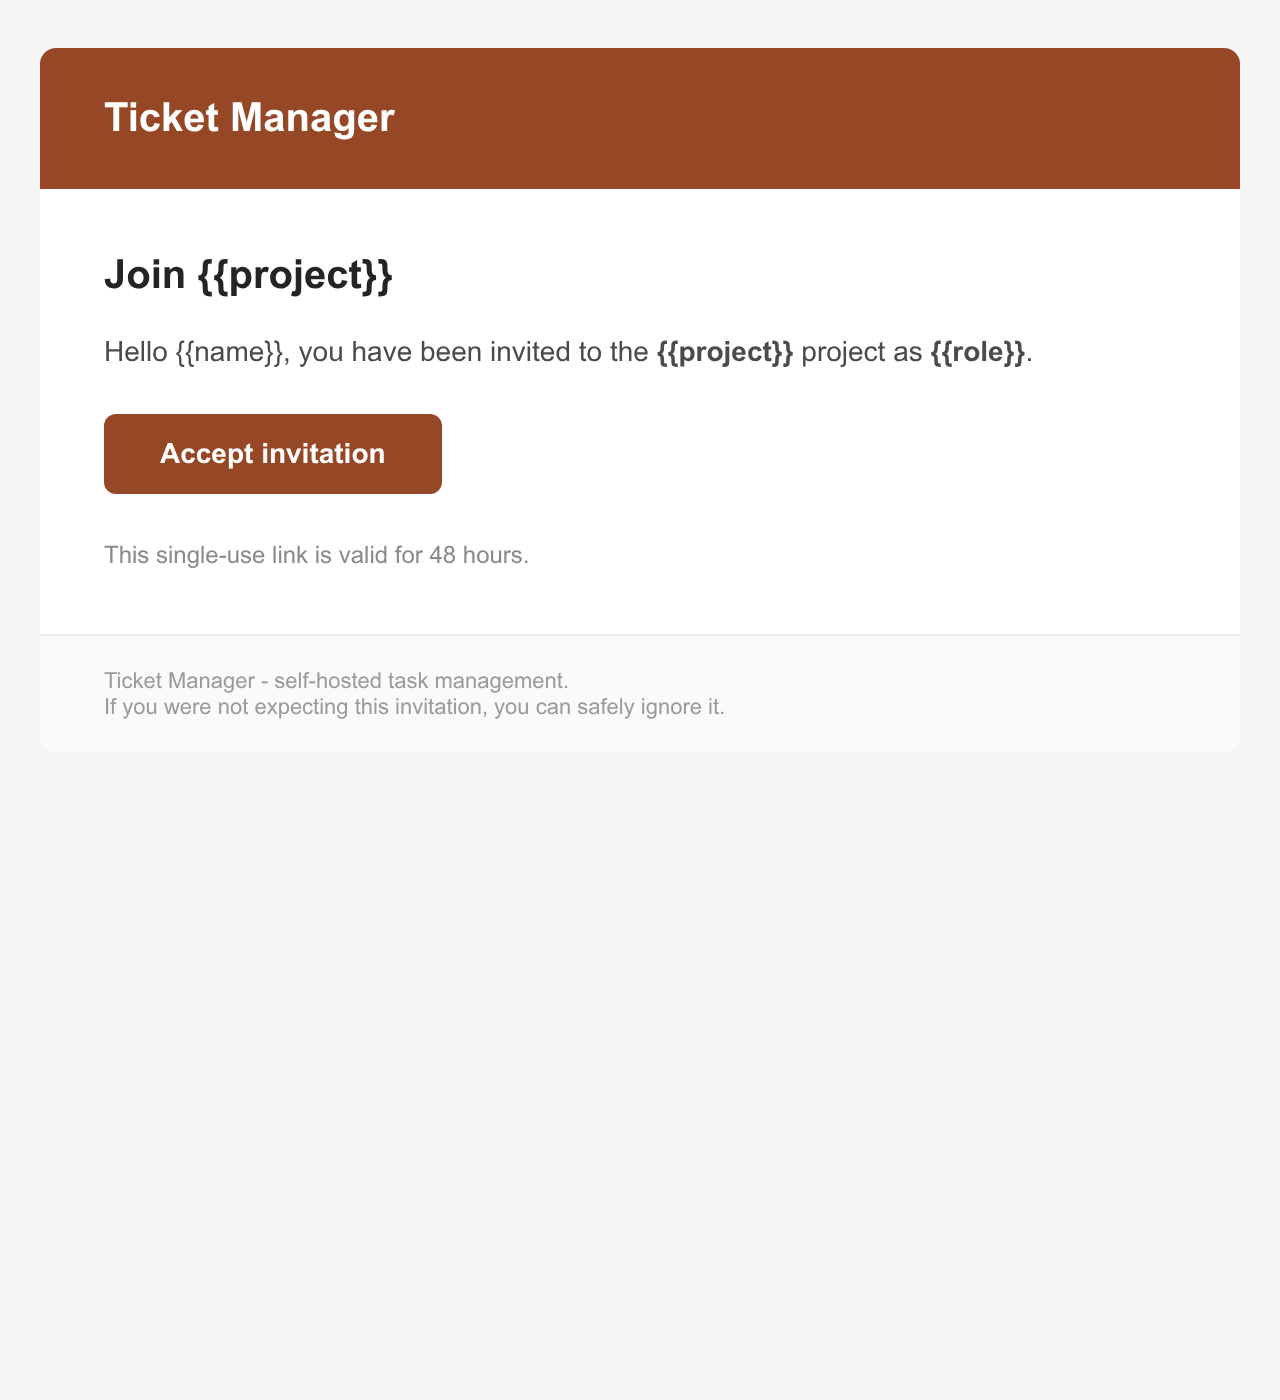
\includegraphics[width=\dimexpr\linewidth-8pt\relax]{templates/preview-invite.png}}\\[4pt]
  {\footnotesize\texttt{invite.html}}
\end{minipage}\hfill
\begin{minipage}[t]{0.48\textwidth}
  \centering
  \fcolorbox{darkgray}{white}{%
    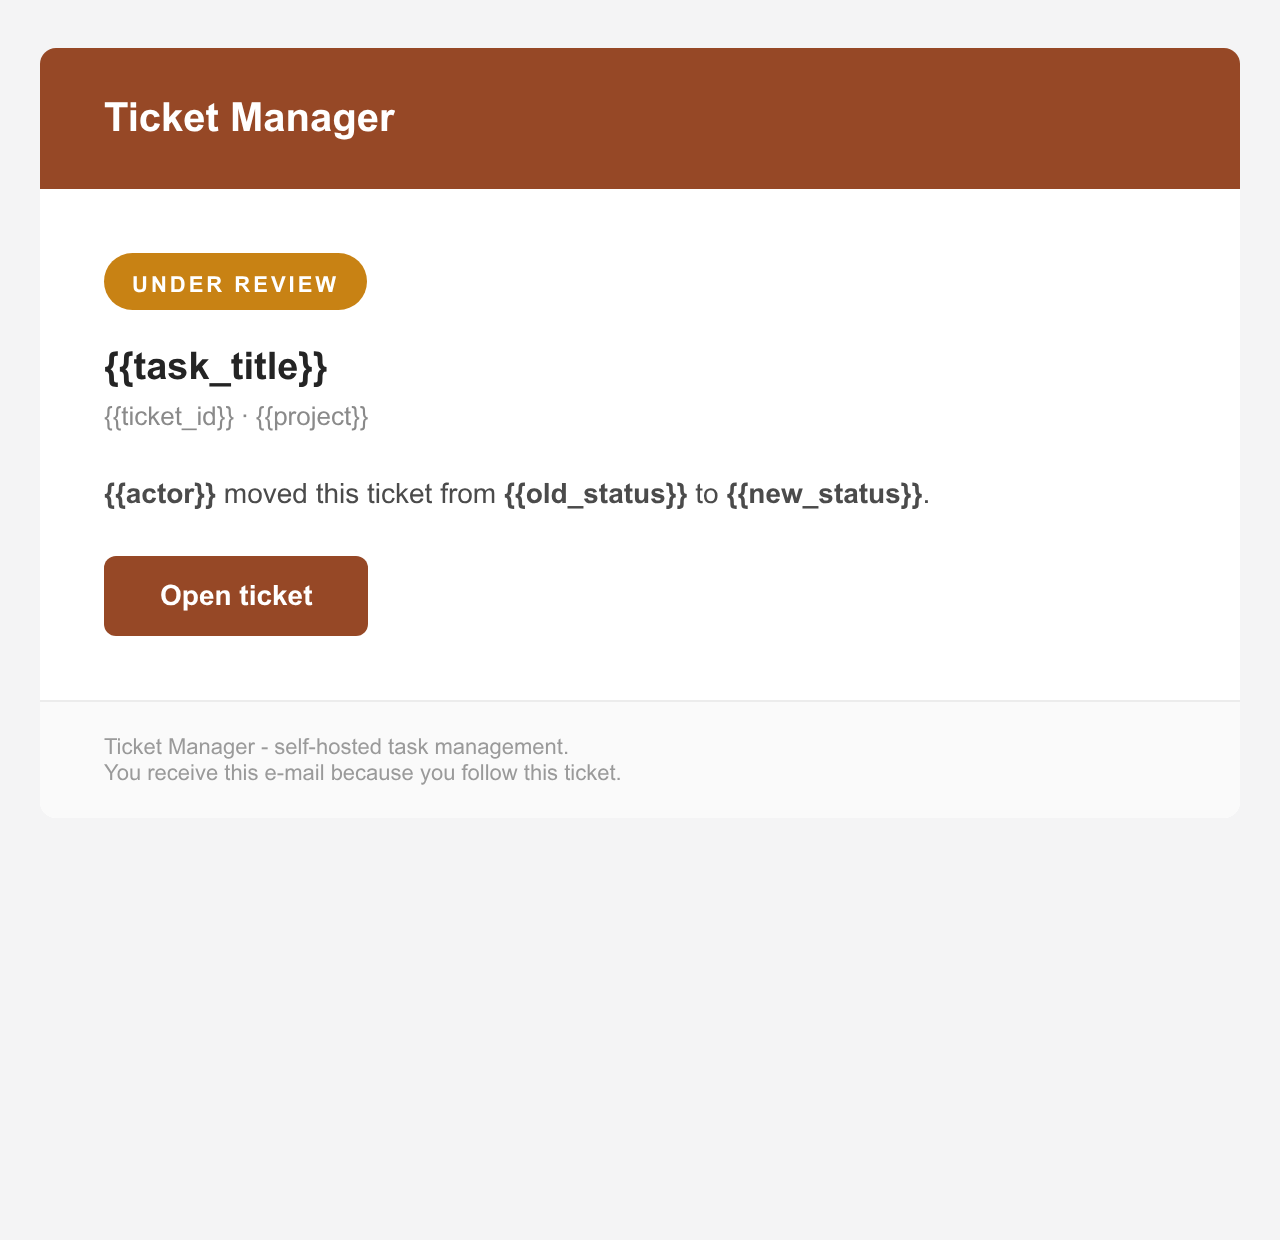
\includegraphics[width=\dimexpr\linewidth-8pt\relax]{templates/preview-status.png}}\\[4pt]
  {\footnotesize\texttt{status-under-review.html}}
\end{minipage}}
\caption{Şablonların 600px e-posta genişliğindeki tarayıcı önizlemesi.}
\label{fig:sablonpreview}
\end{figure}

\lstinputlisting[style=html,
                 caption={Davet e-postası şablonunun tam kaynağı (\texttt{templates/invite.html})},
                 label={lst:invite}]
                {templates/invite.html}

% ============================================================
\section{Güvenlik ve Dayanıklılık Notları}
\label{sec:guvenlik}

\begin{itemize}
  \item \textbf{Sunucu tarafı yetkilendirme:} Her API isteğinde oturum
  geçerliliği ve proje üyeliği doğrulanır; nesne kimlikleri üzerinden
  yetkisiz erişim (IDOR) denemeleri bu katmanda engellenir.
  \item \textbf{Sır yönetimi:} Resend API anahtarı gibi sırlar
  \texttt{wrangler secret} ile yönetilir; depoda düz metin kimlik
  bilgisi bulunmaz.
  \item \textbf{Davet tokenları:} Üretim, özetlenerek saklama ve tek
  kullanımlık politikalar Bölüm~\ref{sec:davit}-te açıklanmıştır.
  \item \textbf{Idempotent cron işleri:} Her koşu bir periyot damgası
  kaydeder; aynı zaman penceresi için ikinci gönderim yapılmaz. Böylece
  beklenmedik yeniden çalıştırmalar çift e-posta üretmez.
  \item \textbf{Şema düzeyi garantiler:} \texttt{tasks.ticket\_id}
  üzerindeki \texttt{UNIQUE} kısıtı, uygulama katmanındaki atomik sayaç
  yaklaşımının arkasındaki son savunma hattıdır.
\end{itemize}

\subsection{Açık Tarama ve Raporlama}

Güvenlik açıkları yalnızca tasarım aşamasında değil, yaşam döngüsü
boyunca düzenli olarak taranır ve bulgular ilgili kişilere bildirilir.

\begin{itemize}
  \item \textbf{Bağımlılık taraması:} CI hattında her derlemede
  \texttt{npm audit} çalıştırılır; GitHub Dependabot güncellemeleri
  otomatik öneri olarak açar. Sürümler kilitli lockfile üzerinden
  yönetilir.
  \item \textbf{Sır taraması:} Depoya anahtar sızmasını önlemek için
  commit aşamasında ve CI'da gitleaks benzeri bir tarayıcı ile düz
  metin kimlik bilgileri aranır.
  \item \textbf{Haftalık açık raporu:} Cron Trigger, projede kullanılan
  paketleri OSV açık veritabanına karşı sorgular; kritik ve yüksek
  önem derecesindeki bulgular, \texttt{security-report.html} şablonuyla
  Super Admin'e e-posta ile bildirilir. Raporda etkilenen paket, açık
  kimliği (CVE), önem derecesi ve önerilen düzeltme sürümü yer alır.
  \item \textbf{Bulgu takibi:} Gönderilen raporların özeti uygulama
  tarafında saklanır; düzeltme sürümü deploy edildikten sonra bulgu
  kapatılarak aynı açığın tekrar raporlanması engellenir.
\end{itemize}

% ============================================================
\section{Sürüm Geçmişi}

\begin{table}[H]
\centering
\small
\begin{tabularx}{\textwidth}{p{1.6cm}p{3.2cm}X}
\toprule
\textbf{Sürüm} & \textbf{Tarih} & \textbf{Notlar}\\
\midrule
v0.1 & ---     & İlk mimari taslağı.\\
v0.2 & \today  & Şema sıkılaştırıldı (UNIQUE kısıtları, atomik sayaç, indeksler); yetki ve bildirim matrisleri eklendi; güvenlik bölümü eklendi.\\
\addlinespace
v0.3 & \today  & Yönetim paneli için react-admin kararı; MailHog tabanlı geliştirme ortamı ve durum bazlı HTML e-posta şablonları; açık tarama ve raporlama bölümü eklendi.\\
\addlinespace
v0.4 & \today  & Şablon örnekleri depoya eklendi (\texttt{templates/}); rapora şablon kaynak kodu ve tarayıcı önizlemeleri dahil edildi; hedef konumlandırma (öz-sunumlu Linear alternatifi) netleştirildi.\\
\addlinespace
v0.5 & \today  & Ürün adı Ticket Manager olarak netleştirildi; PlannedLost ile ilişki konumlandırması düzeltildi; şablon marka başlıkları güncellendi.\\
\bottomrule
\end{tabularx}
\caption{Doküman sürüm geçmişi.}
\end{table}

\end{document}
